% filepath: report/4-rule.tex
\section{Rule Modification}
To encourage forward progress and strategic multi-jumping, we modified the rule and applied full experiments on it.

\subsection{Revised Experimental Setup}

We introduced two new parameters to encourage progress.
\begin{itemize}
  \item Maximum turns: 100.  
    If a match exceeds 100 turns, it ends in a draw to prevent score exploits through repetitive movements.
  \item Goal entry reward: 10 points per pawn entering the goal.
  \item Jump reward scalar (\texttt{jump\_scalar}):  
    For a sequence of \texttt{jump\_count} consecutive jumps, award \(\texttt{jump\_count} \times \texttt{jump\_scalar}\) additional points.
\end{itemize}

We first evaluate \(\texttt{jump\_scalar}\in\{1.0,1.2,1.5,2.0,5.0\}\), then conduct a binary search to find the value yielding roughly 50\% draws.

In Part (1) of the experiment, we evaluate agent performance under five different values of \texttt{jump\_scalar}: 1.0, 1.2, 1.5, 2.0, and 5.0. In Part (2), we apply a binary search strategy to determine the optimal value of \texttt{jump\_scalar} that results in approximately 50\% of the matches ending in a draw.

\subsection{Revised Winning Condition}

\begin{itemize}
  \item If all pawns enter goal areas within 100 turns, the higher-scoring player wins.
  \item Otherwise, the match is a draw.
\end{itemize}

\subsection{Revised Experiment Results}
Under the revised settings and winning conditions, we conducted head-to-head matches for Greedy, Minimax and Minimax Local Search players. Note that we limit our evaluation to G, M, and MLS, as other agent types are unable to fully exploit the additional rewards introduced by the revised rules. The outcomes of these matches are summarized and visualized using heatmaps to highlight win rates and performance differences across agents.

The revised results in part (1) are illustrated in the first five subplots in Figure~\ref{fig:jump}, where each cell indicates the win rate (in percentage) of the first player (Sente, row) when playing against the second player (Gote, column).

For clarity, the agents are abbreviated as follows: G (Greedy), M (Minimax), MLS (Minimax Local Search).

\begin{figure}[h]
    \centering
    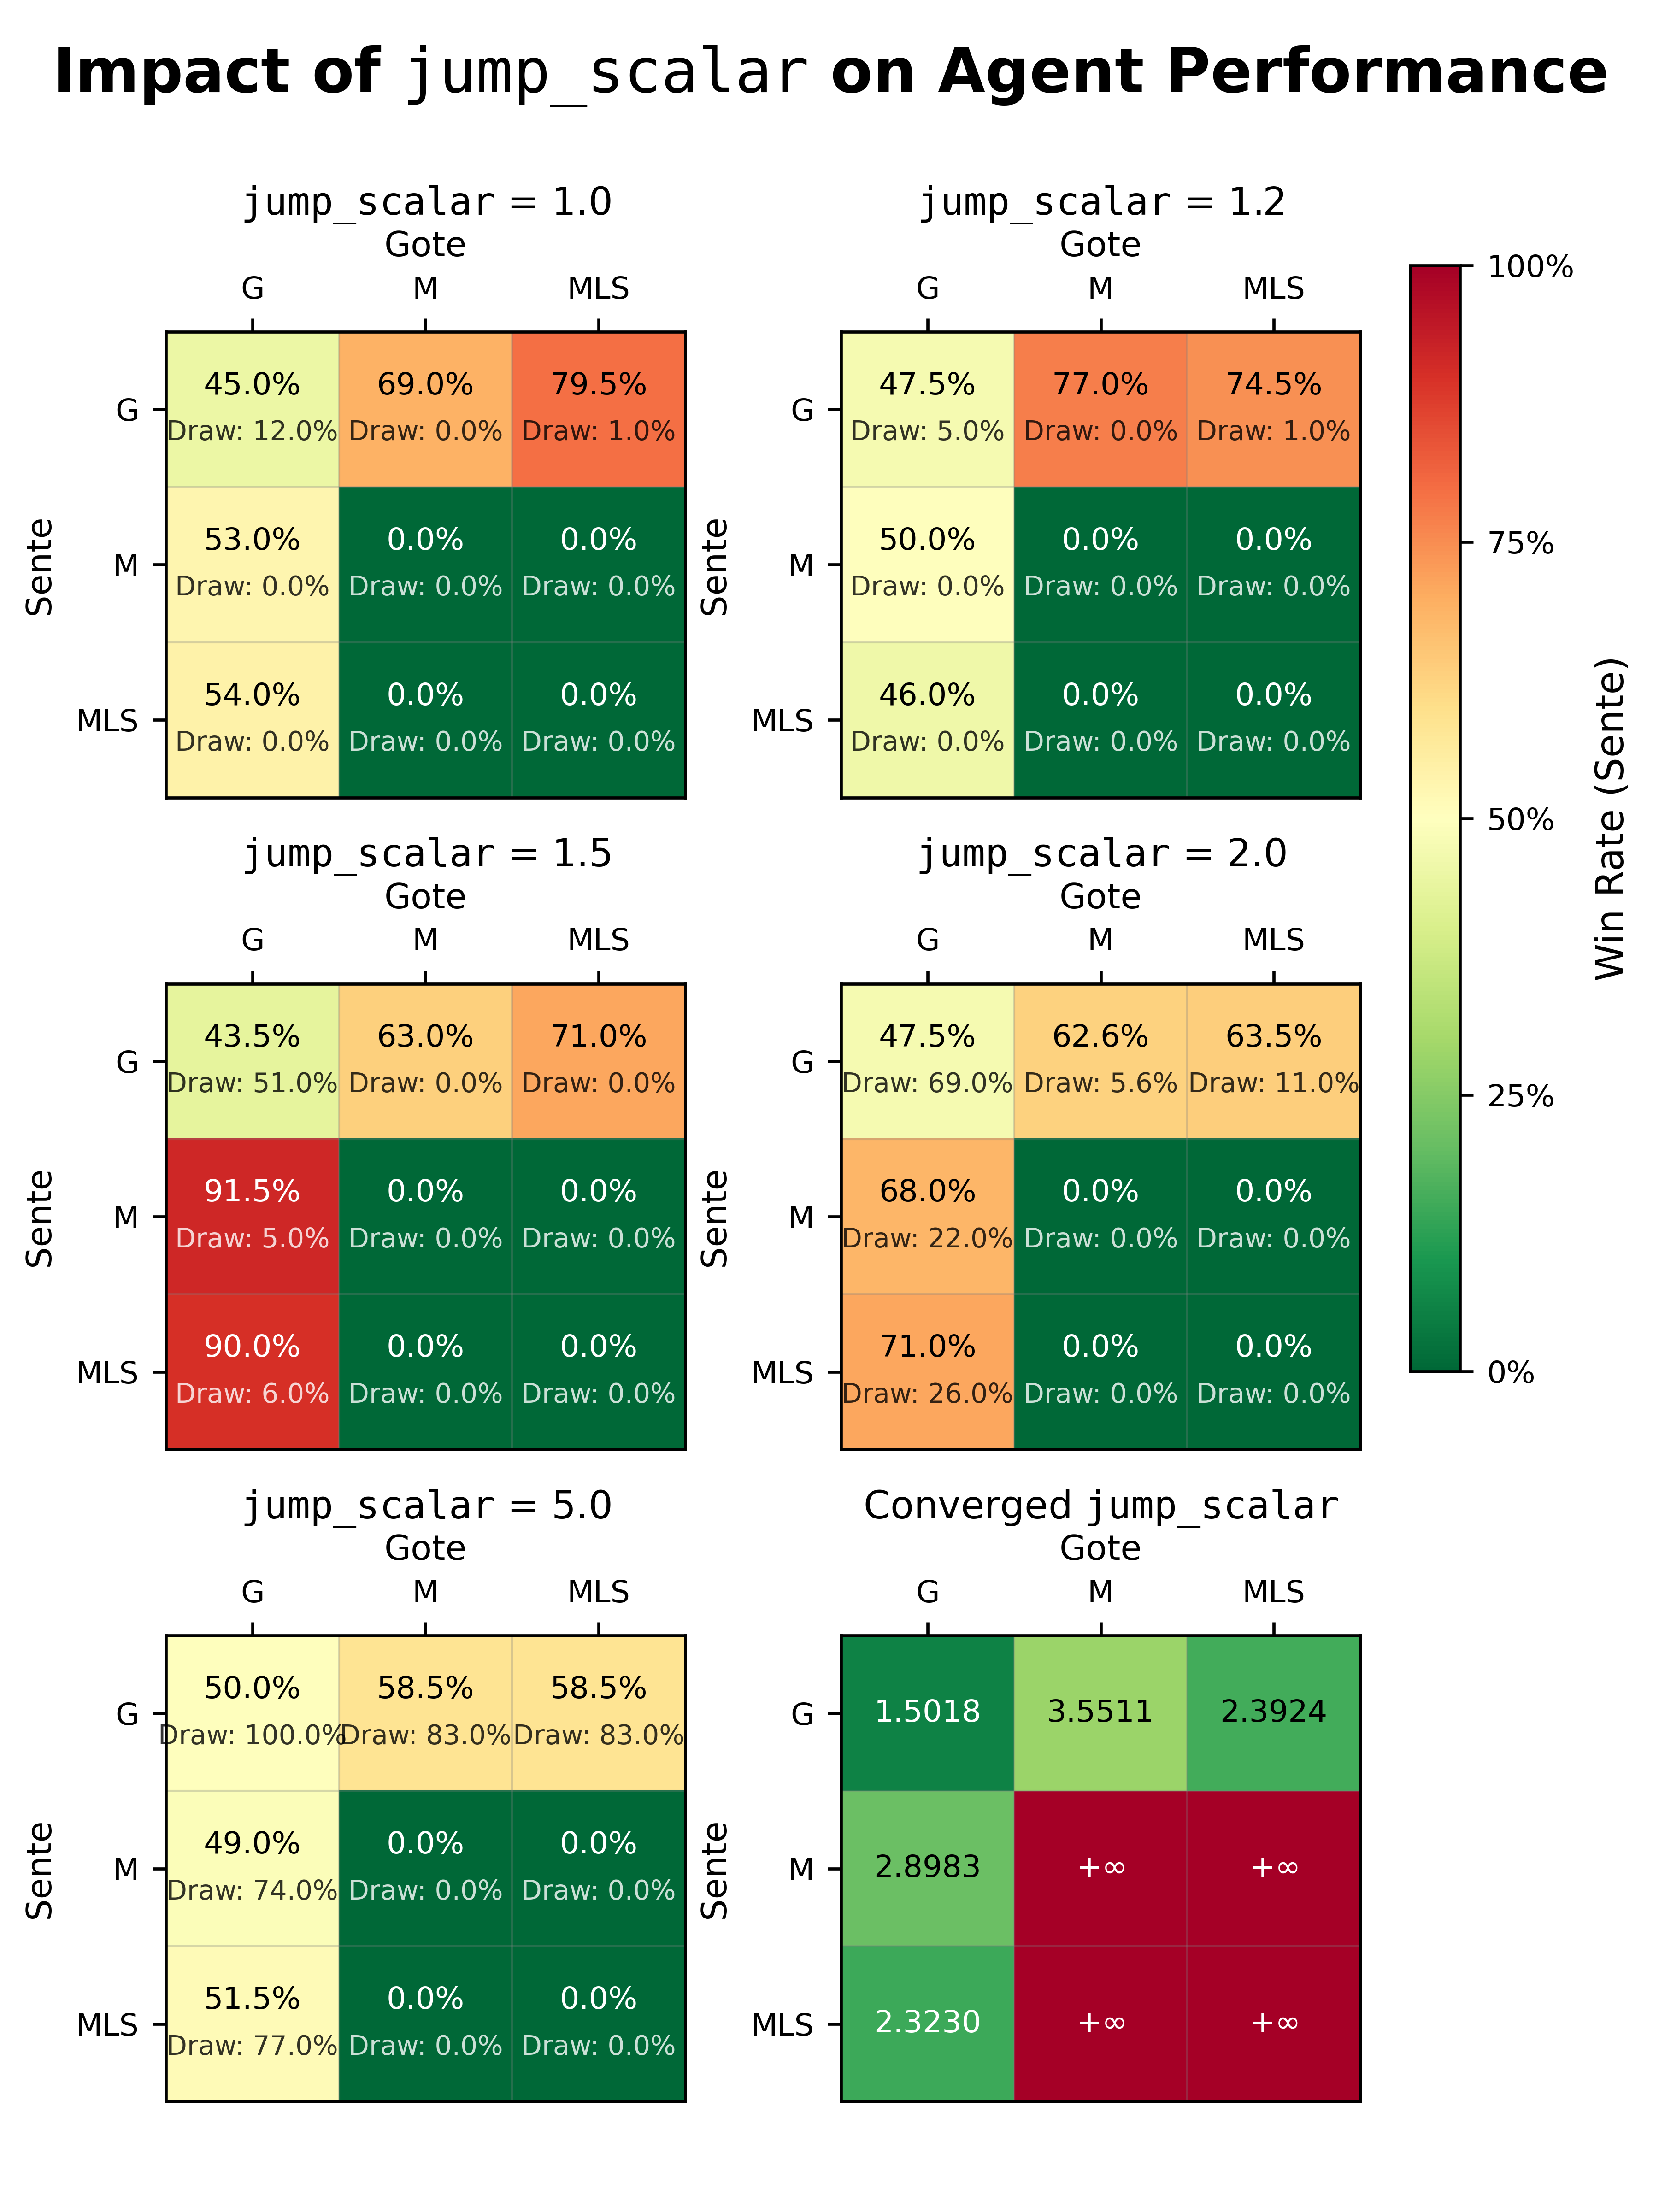
\includegraphics[width=1\columnwidth]{figures/jump_scalar.png}
    \caption{Impact of \texttt{jump\_scalar}}
    \label{fig:jump}
\end{figure}